\section{Preliminary Design}
\label{sec:preliminary_design}
%\subsection{Preliminary Design Explanation}
%Explain the preliminary design including block diagrams, schematics, drawings, etc.
%Modular design - easy for scaling
%Output voltage level trade analysis
%Analysis of "orbit"
%Component ratings considerations
%Possible up-scaling of system - larger power, modular design, higher voltage?
%Load profile/switching: motors, communication, payload(s), OBDH?, sensors, regulators?,
%Decide on sufficient design margins?
%EMI/EMC/ESD for scientific payloads and safety
%Look into previously flown solar powered airships
%Scalability to fly in high-altitude "orbits" i.e. temperatures, reliability, ionization?, 
%Possibility to cover "wings" with solar cells - trade study of benefit!
%Payload short-circuit
%
\subsection{Solar Array Design}
%Bypass diodes on SA to mitegate shadowing problems
%Cross-strapping of solar cells?
%\subsubsection*{Solar Array Shading}
%Bypass diodes can be used to partly mitigate this issue as well as using \ac{MPPT}. Otherwise it could be necessary to ensure that the airship structure cannot cast shadows on the panels and that the airship only fly above or away from landscape objects.
%SA isolation diodes
%
Section \ref{subsec:environmental_requirements} discussed the importance of the sun incidence angle on the solar panels. It is first considered having the solar array divided into two identical panels on each side of the airship. Considering that the sun incidence is directly falling on one of the sides of the airship, the "back-side" solar panel on the airship may still produce power, if the incidence angle is not too large. Considering the Kelly cosine function from figure \ref{fig:KellyCosine}, the maximum total output current (power), from each solar panel, is around $71\%$, when both solar panels are at $90^{\circ}$ angles (completely flat on top of the airship). In practical, having complete flat panels on top of the airship is hard to realize and a compromise must be made. Hence, the panels should be angled as small as possible, to maximize the total power output.

The same issue goes for the changing sun incidence angle due to the flight attitude around the vertical axis. Again, ideally the solar panels should be flat on the top of the airship. In practical, it is more realistic to place four identical solar panels on top of the airship, with as small an angle as possible with respect to vertical. The proposed layout of the four solar panels is illustrated in figure \ref{fig:solar_panels_mounting}.
%
\begin{figure}[H]
\centering
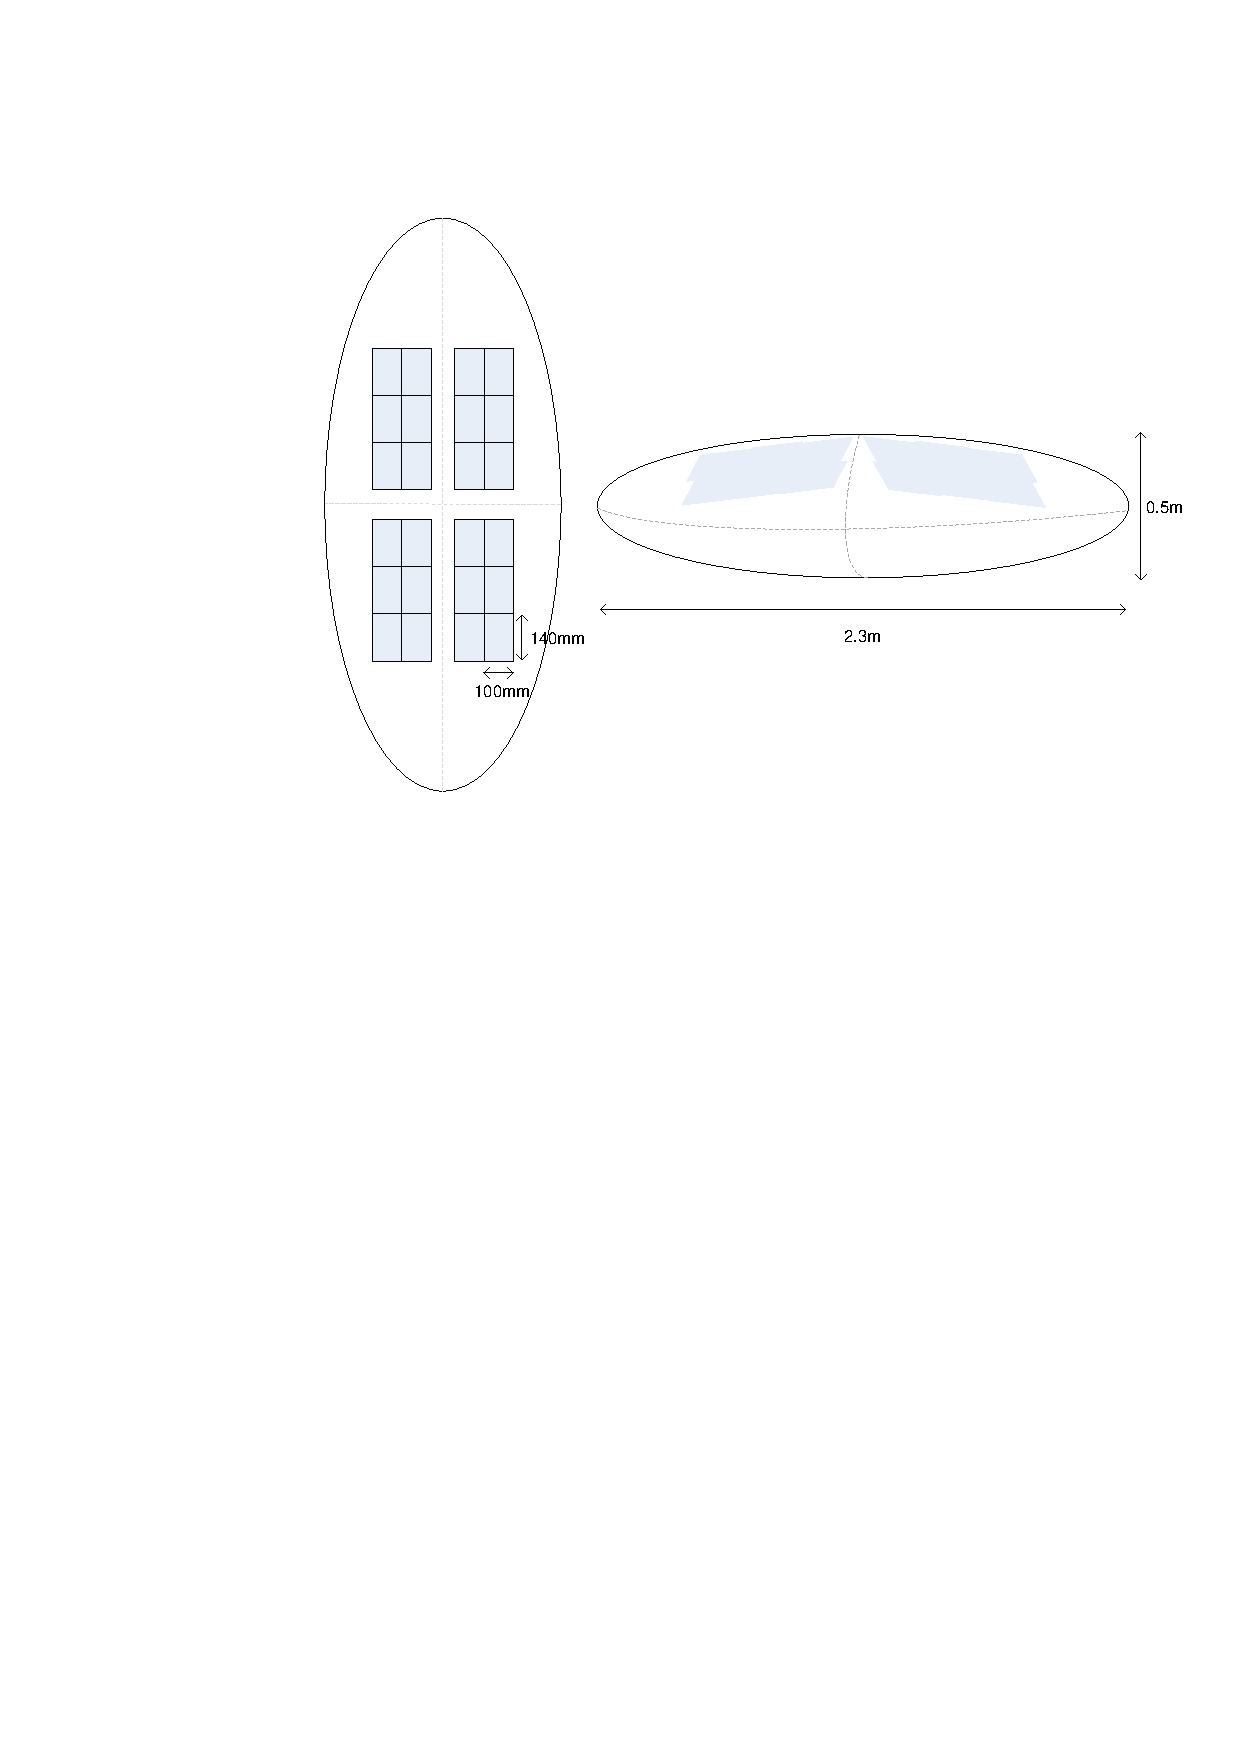
\includegraphics[scale=0.8]{figures/fig_PDR_Solar_Panels_Mounting}
\caption{Mounting of the solar panels}
\label{fig:solar_panels_mounting}
\end{figure}
%
The proposed solar cell, \cite{MC_Solar_Cell}, has the following current and voltages at the \ac{MPP}:
%
\begin{equation}
\begin{split}
V_{cell,MPP}&=3.85\,V\\
I_{cell,MPP}&=210\,mA
\end{split}
\end{equation}
%
Each of the four panels will consist of six solar cells giving a maximum power output of:
%
\begin{equation}
\begin{split}
P_{panel,MPP}&=6\cdot V_{cell,MPP}\cdot I_{cell,MPP}\\
P_{panel,MPP}&=4.85\,W
\end{split}
\end{equation}
%
It is considered having two series-connected cells and three in parallel, thus having an output voltage of: 
%
\begin{equation}
V_{panel,out}=7.7\,V
\end{equation}
%A future upgrade of the project, could including a simple solar array drive mechanism for each solar panel. This could increase the solar arrays output and make the design more flexible for flying in varying solar incidence angles, i.e. different seasons, latitudes or time of day. However, this approach is more complicated and not applicable for the U-SPACE project.
%

%
\subsection{Regulator Design}
%Which design concepts are considered? - What are the advantages/disadvantages for each concept?
%Decide on MPPT algorithm (using analog circuits?)
%DC-DC regulator topology (Buck, Boost, Buck-Boost etc.)
%
%
An important trade-off analysis is the selection of the \ac{SAR}. Table \ref{tab:TradeOff} shows the comparison between three possible regulators. These three are shortly described below:
%
\subsubsection*{Zener Diode Regulator}
The most simple design is to use a Zener-diode regulator, as shown in figure \ref{fig:zenerdiode_regulator}. The circuit comprises a Zener-diode with a reverse break-down voltage equal to the desired output voltage. Excessive current from the solar arrays runs through the Zener-diode, thus keeping the load current and output voltage constant. The resistor is included to limit the current drawn by the Zener-diode to protect it from over-currents. Since a series resistor is inserted, significant  power losses are experienced and therefore this circuit is only useful in low power applications. 
%
\begin{figure}[H]
\centering
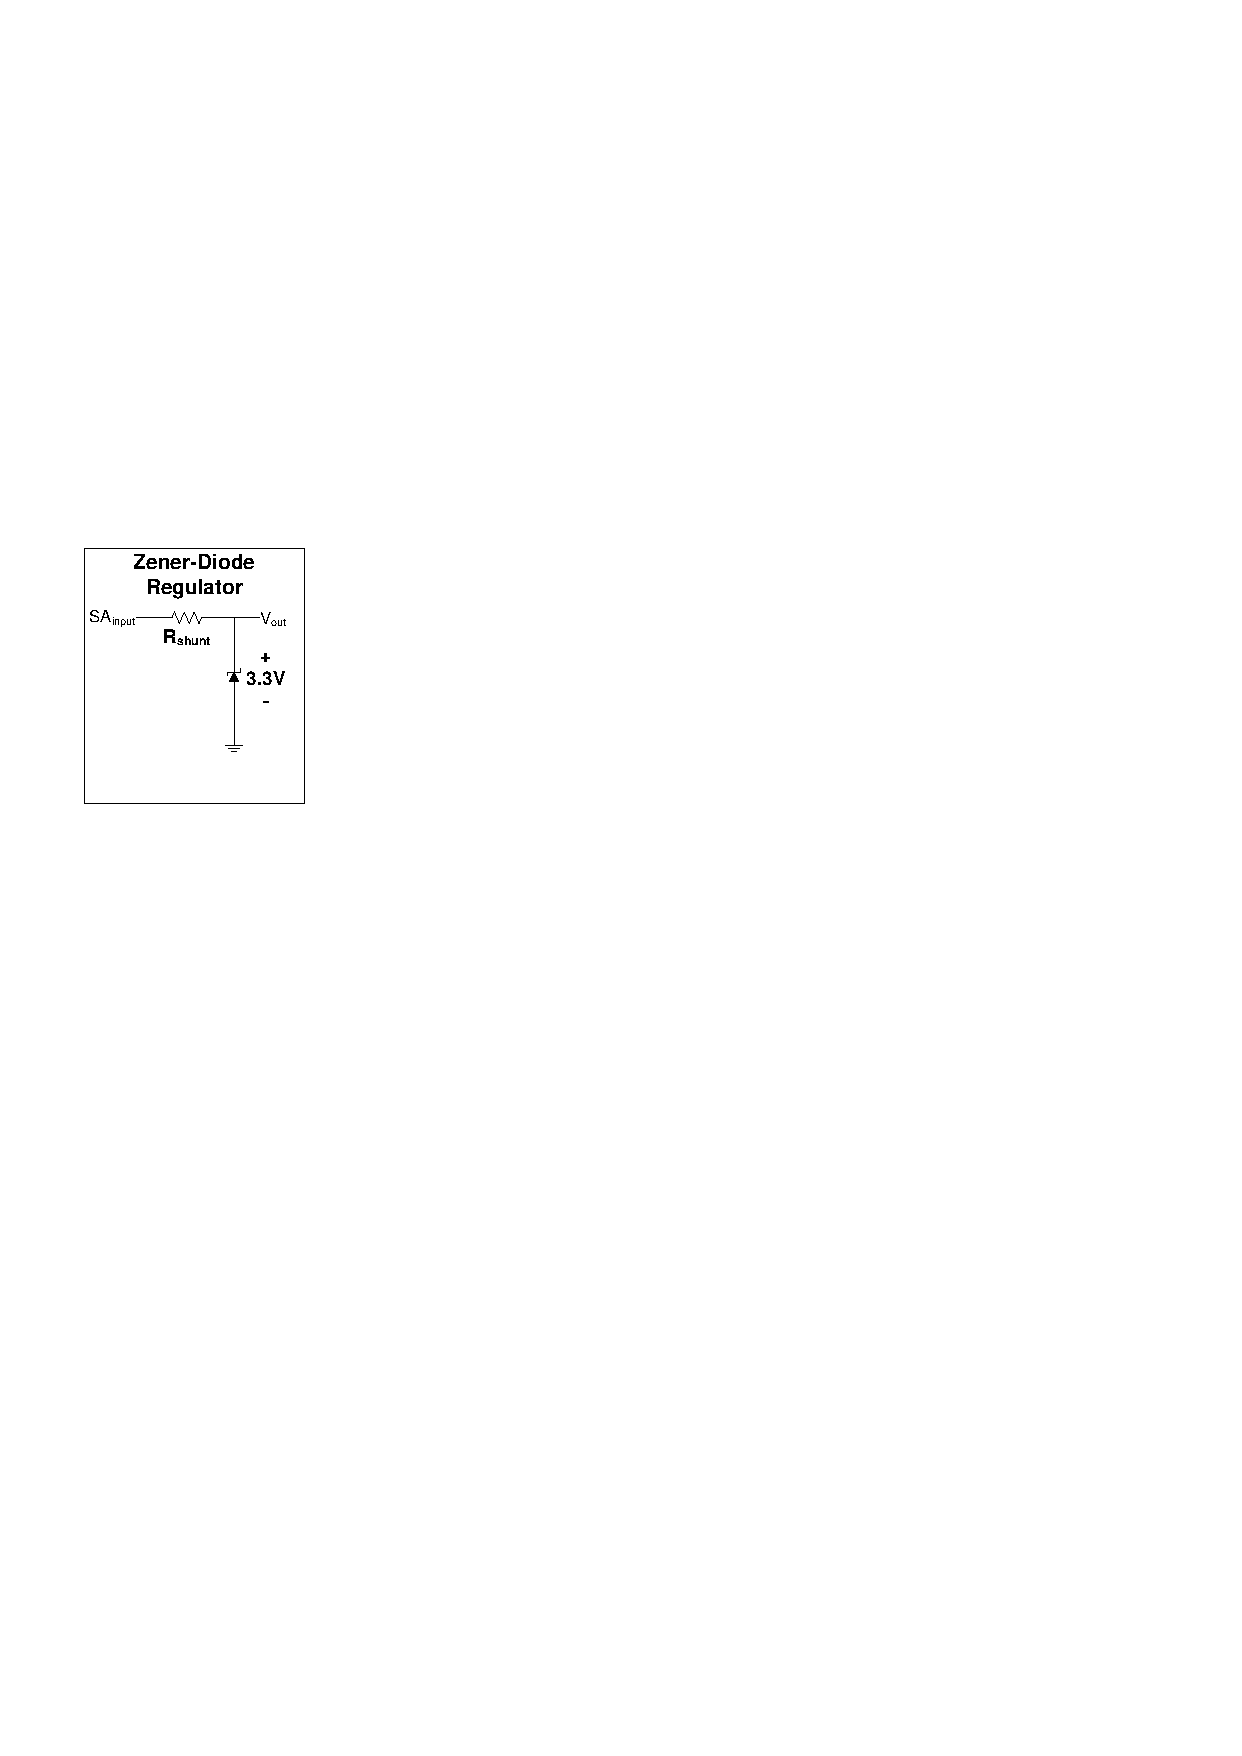
\includegraphics[scale=1]{figures/fig_PDR_Zenerdiode_Regualtor}
\caption{Simple Zener-diode regulator}
\label{fig:zenerdiode_regulator}
\end{figure}
%
%
\subsubsection*{Shunt Regulator}
The shunt regulator concept also uses a shunt resistor, but the Zener-diode is replaced by a transistor. When the transistor is closed, the solar array current is shorted to ground through the shunt resistor. A feedback line measures the output voltage, compares it to a reference voltage and generates a control signal. This signal is fed to a \ac{PWM} driver for the transistor gate. This way, the current supplied to the load can be controlled and the output voltage kept constant. The solar array will operate at the same voltage as the output voltage. By manually changing the reference voltage, the output voltage could be changed, thus adding some degree of flexibility for operating conditions of the solar array. The shunt-regulator concept is shown in figure \ref{fig:shunt_regulator}.
%
\begin{figure}[H]
\centering
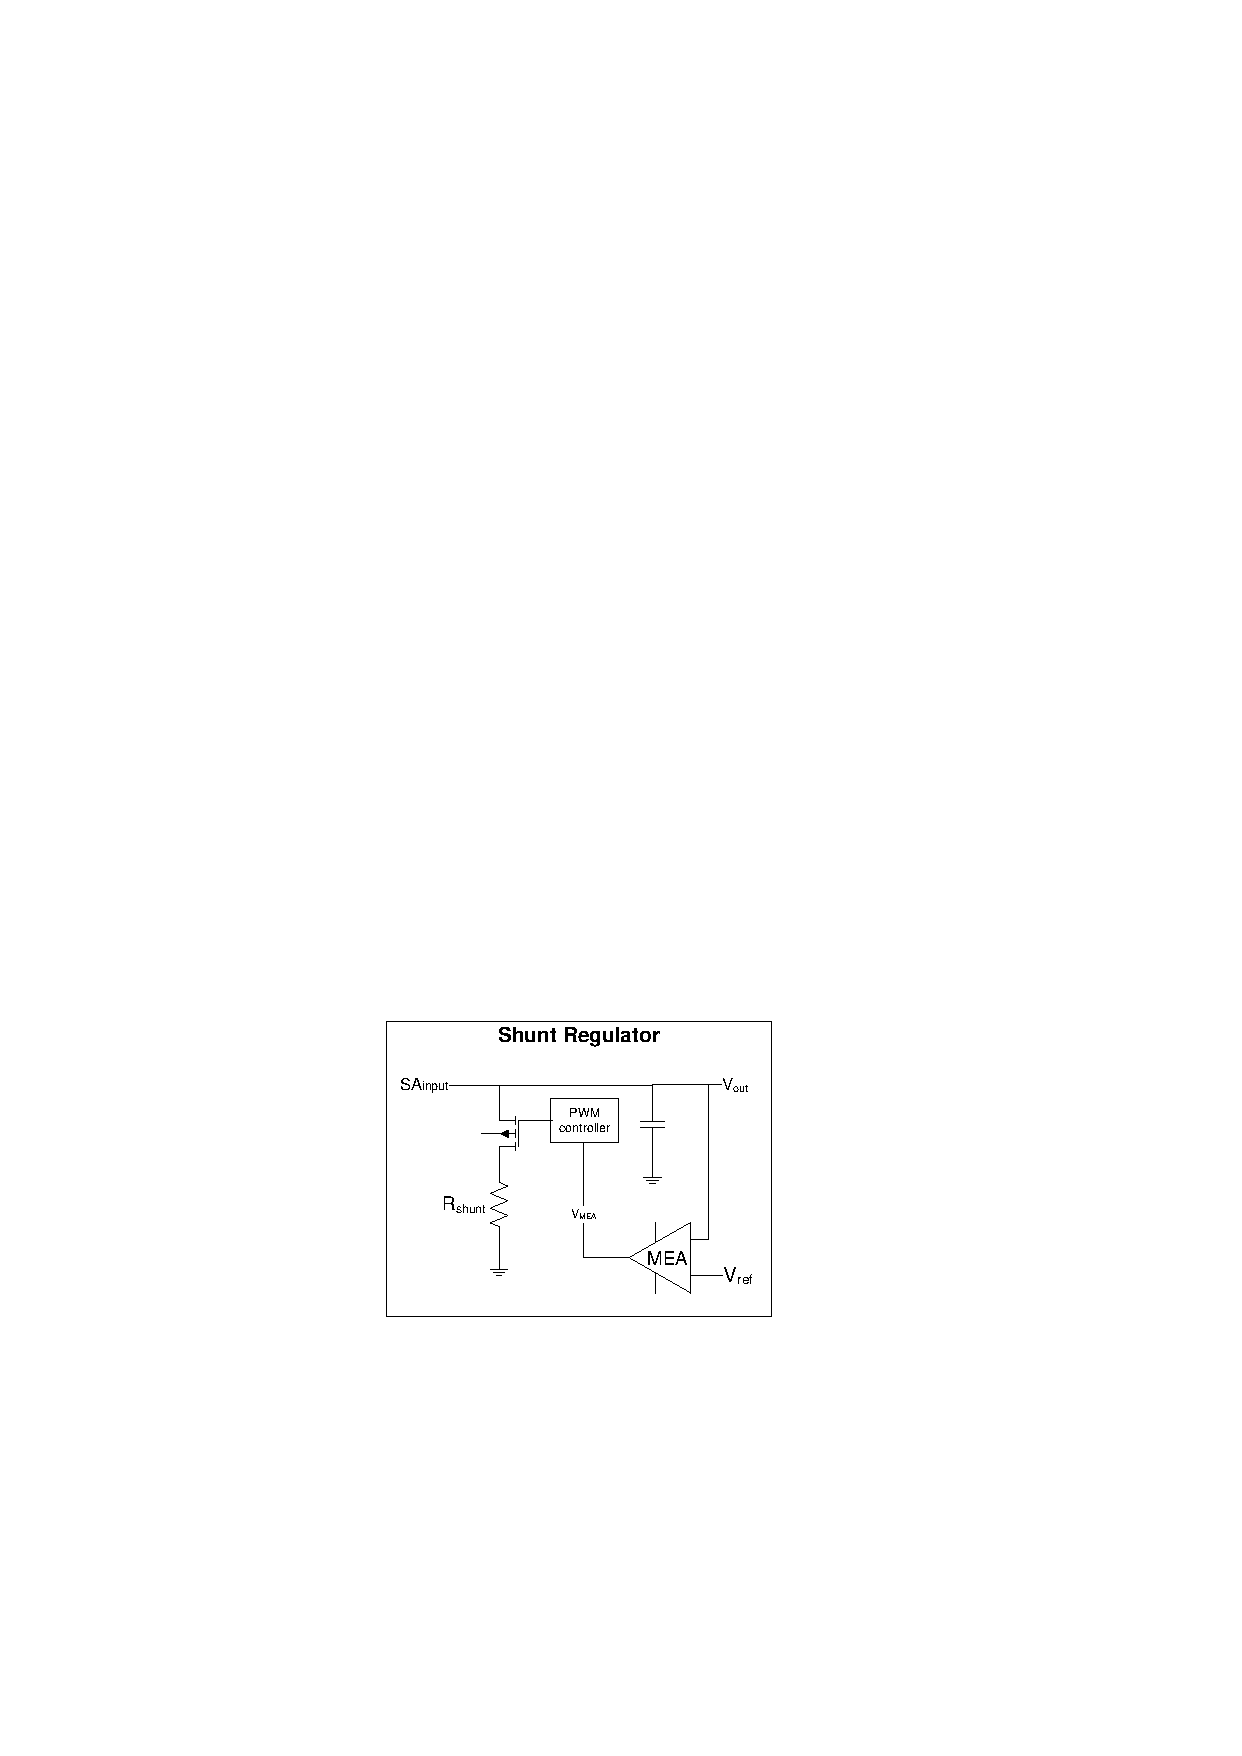
\includegraphics[scale=1]{figures/fig_PDR_Shunt_Regulator}
\caption{Shunt regulator diagram}
\label{fig:shunt_regulator}
\end{figure}
%
\subsubsection*{Maximum Power Point Tracking Regulator}
The most advanced and robust solution is to use an \ac{MPPT} regulator as shown in figure \ref{fig:MPPT_regulator}. A standard DC-DC converter topology (buck or boost) is used, comprising a transistor, free-wheel diode, inductor and output capacitor. Like in the shunt-regulator, the output voltage is measured and compared to a reference voltage, to generate a \ac{PWM} control signal, to drive the transistor. By varying the duty cycle of the \ac{PWM} signal, the input voltage (solar array operating voltage) can be controlled. Additionally an \ac{MPPT} circuit is added. The solar array current and voltage are measured and fed to the circuit which then calculates the power output of the solar array. By making small steps in the solar array operating voltage, the characteristic IV-curve of the solar array can be generated and the \ac{MPP} can be tracked, thus always operating the solar array at is optimal operating point. When using an \ac{MPPT} regulator, three operating modes will be possible:
%
\begin{itemize}
\item Battery discharge {MPPT} - when the solar array input power is insufficient to cover the load power demand, the battery is slowly discharged in order to maintain the output voltage.
\item Battery charge {MPPT} - when the solar array input is greater than the load power, the excessive power is used to recharge the battery.
\item Input power limitation - when the battery is fully charged, the regulator will operate the solar array at a non-optimal voltage, thus limiting the input power to keep the output voltage constant. The extra potential input power is dissipated as heat externally on the solar arrays.
\end{itemize}
%
\begin{figure}[H]
\centering
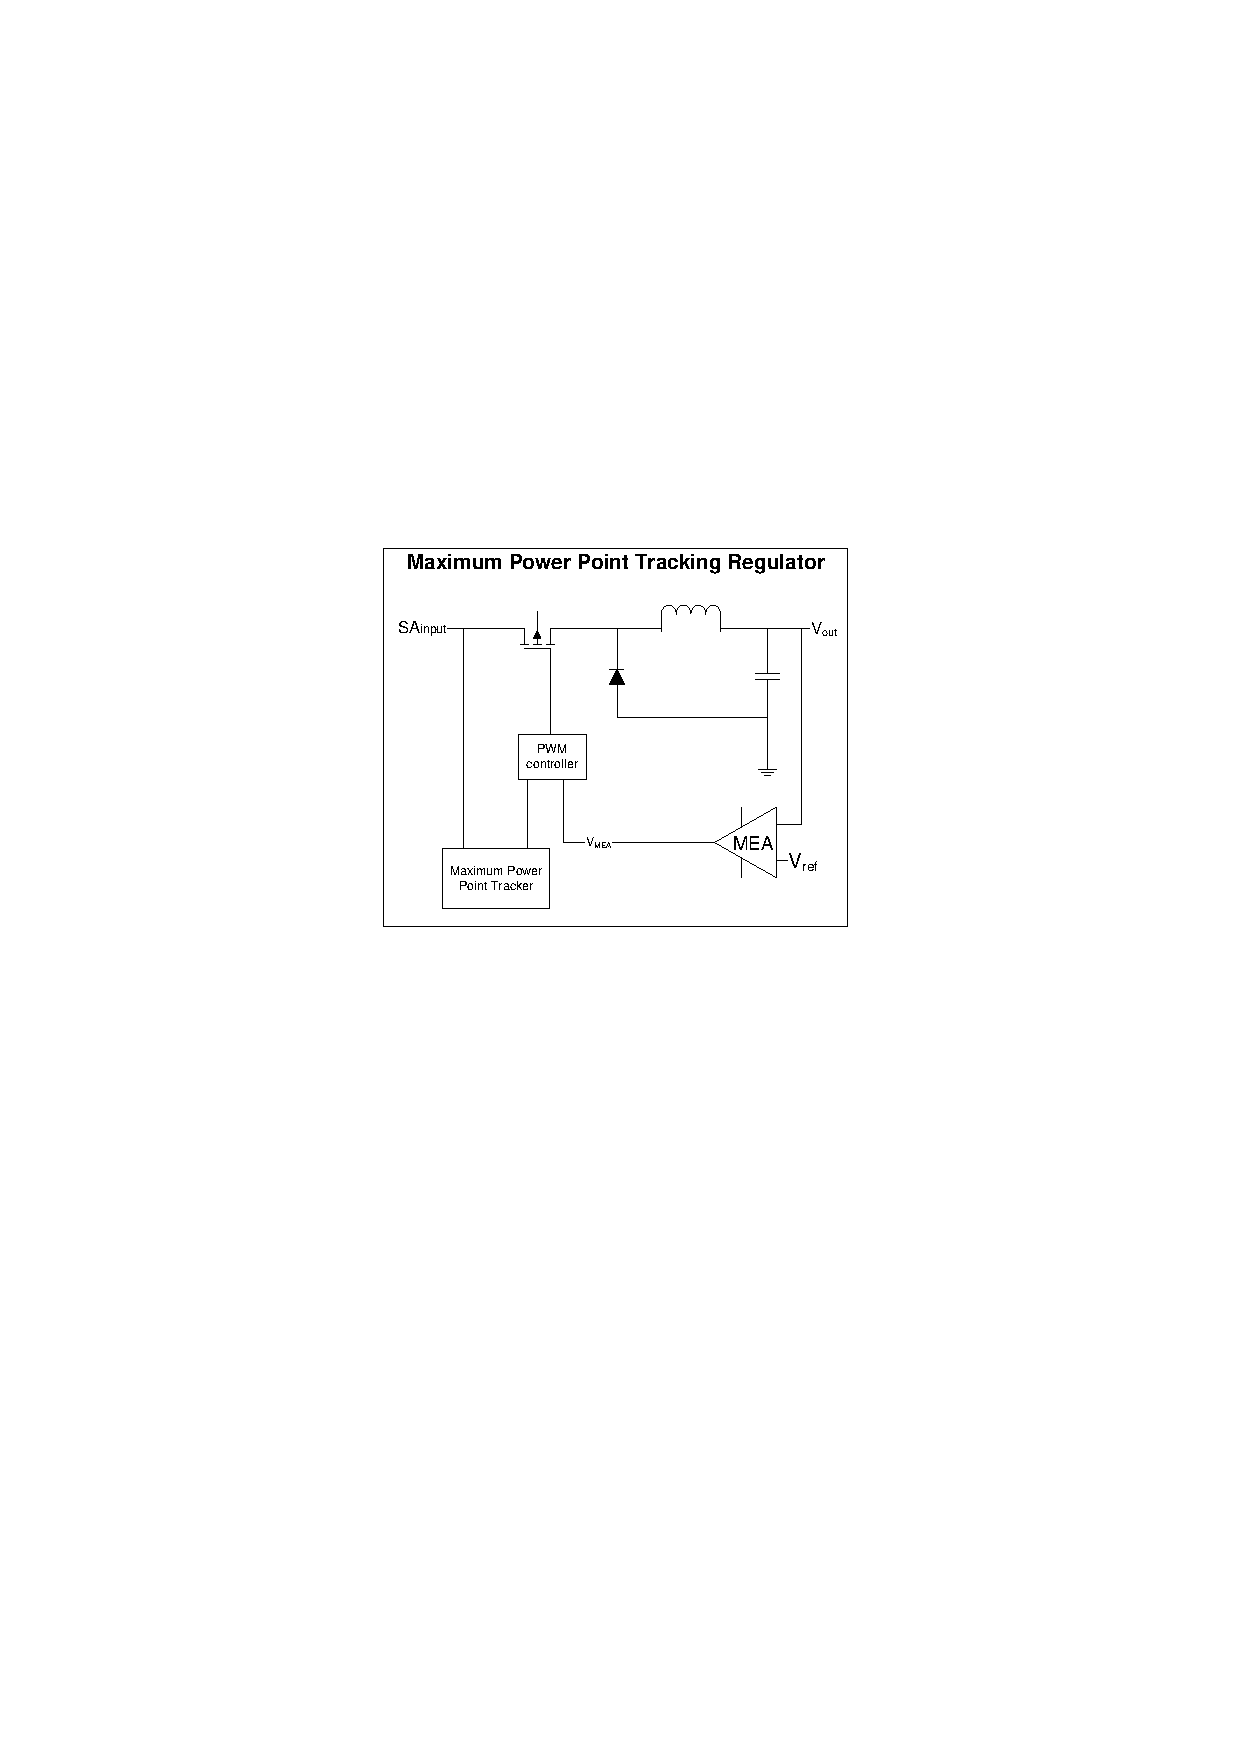
\includegraphics[scale=1]{figures/fig_PDR_MPPTdiagram}
\caption{\ac{MPPT} regulator diagram}
\label{fig:MPPT_regulator}
\end{figure}
%
%
%\begin{center}
\begin{table}[H]
\centering
\rowcolors{3}{tableshade}{white}
\caption{Trade off analysis}
\label{tab:TradeOff}
\begin{minipage}{\textwidth}
\centering
\begin{tabular}{||p{0.22\textwidth}p{0.22\textwidth}p{0.22\textwidth}p{0.22\textwidth}||}
\hline
\textbf{SA Regulator Concepts:} &  \textbf{MPPT} & \textbf{Shunt-Regulator} & \textbf{Zener-diode Regulation}\\ 
\hline
Costs & Medium(some ICs required) & Medium(some ICs required) & Low(simple components)\\
Regulator efficiency & High($90-95\%$) & Medium($70-95\%$) & Low($40-70\%$\footnote{Efficiency drops significantly at high current loads, due to the shunt resistor})\\
Size/mass & $\sim140-240 g$\footnote{up to four identical circuits are needed, one for each solar panel, hence the larger mass} & $\sim50 g$ & $\sim45 g$\\
Output voltage stability & Good & Average & Poor\\
Scalability & Very good & Average & Poor\\
Internal heat dissipation & Low & Medium & High\\
Complexity & High & Medium & Low\\
Flexible to variations(temperature, shading, degradation) & Very good & poor (only manually) & none\\
Implementation time & $\sim1-2\,months$ & $\sim3-4\,weeks$ & $< 1\,week$\\
\hline
\end{tabular}\par
\vspace{-0.75\skip\footins}
\renewcommand{\footnoterule}{}
\end{minipage}
\end{table}
%\end{center}
%
\subsection{Battery Design}
%
A trade-off analysis between different battery chemistry has been conducted and the results are listed in table \ref{tab:TradeOff_battery}. 
%
%Battery overcharge
%Battery charge limitation
%Battery short-circuit?
%Charge regulation: Bulk, Taper, Trickle-charging.
%Battery maximum charge ratio
%Battery maximum discharge ratio
%Battery maximum Depth of Charge (DOD)
%
%
\begin{center}
\begin{table}[H]
\rowcolors{3}{tableshade}{white}
\caption{Trade off analysis}
\label{tab:TradeOff_battery}
\begin{tabular}{||p{0.1\textwidth}p{0.40\textwidth}p{0.40\textwidth}||}
\hline
\textbf{Battery type} &  \textbf{Advantages} & \textbf{Disadvantages}\\ 
\hline
NiCd & ? & Has memory effect and toxic Cadmium\\
NiH2 &  More robust to over-charge/discharge & Low energy density, high self-discharge rate and the pressurized cell is more dangerous to handle\\
NiMH & No internal pressure, higher energy density and less sensitive to temperature & Cannot deliver high peak power, high self-discharge rate, sensitive to high temperatures and is damaged by over-charging\\
Li-ion & Highest energy density, high charge efficiency and supports high charge/discharge rates due to low internal impedance & Expensive, damaged by over-charging/discharging, sensitive to low temperatures and increased internal impedance at low temperatures\\
AgZn & High specific energy, stable cell voltage during dis-charge & Short life time\\
\hline
\end{tabular}
\end{table}
\end{center}
%
It is proposed to use a Panasonic PA-LN19 Li-ion battery \cite{Panasonic}. The battery has the following important specifications:
%
\begin{table}[H]
\centering
\caption{Specification of proposed battery}
\label{tab:proposed_battery}
\begin{tabular}{ll}
\hline
Battery chemistry & Li-ion\\
Battery voltage & $3.6\,V$\\
Battery capacity & $2.9\,Ah$ / $10.44\,Wh$\\
Weight & $49\,g$\\
\hline
\end{tabular}
\end{table}
%
\subsection{Argumentation for Chosen Concept(s)}
%Why is the chosen concept selected?
%
It is proposed to use the \ac{MPPT} concept, since this provides the most efficient and robust design and easy scales up to a larger system if/when required. It also mitigate design challenges occurring due to varying environment conditions, i.e. temperature, weather etc.

For the battery, Li-ion technology offers the most compact design ensuring low weight and relative high energy capacity.

The complete \ac{EPS} diagram is shown in figure \ref{fig:EPSdiagram}. For providing the $5\,V$ regulated voltage to the payloads, \ac{COTS} DC-DC regulator(s) are used. The battery charging/discharging is controlled by the \ac{SAR}.
%
\begin{figure}[H]
\centering
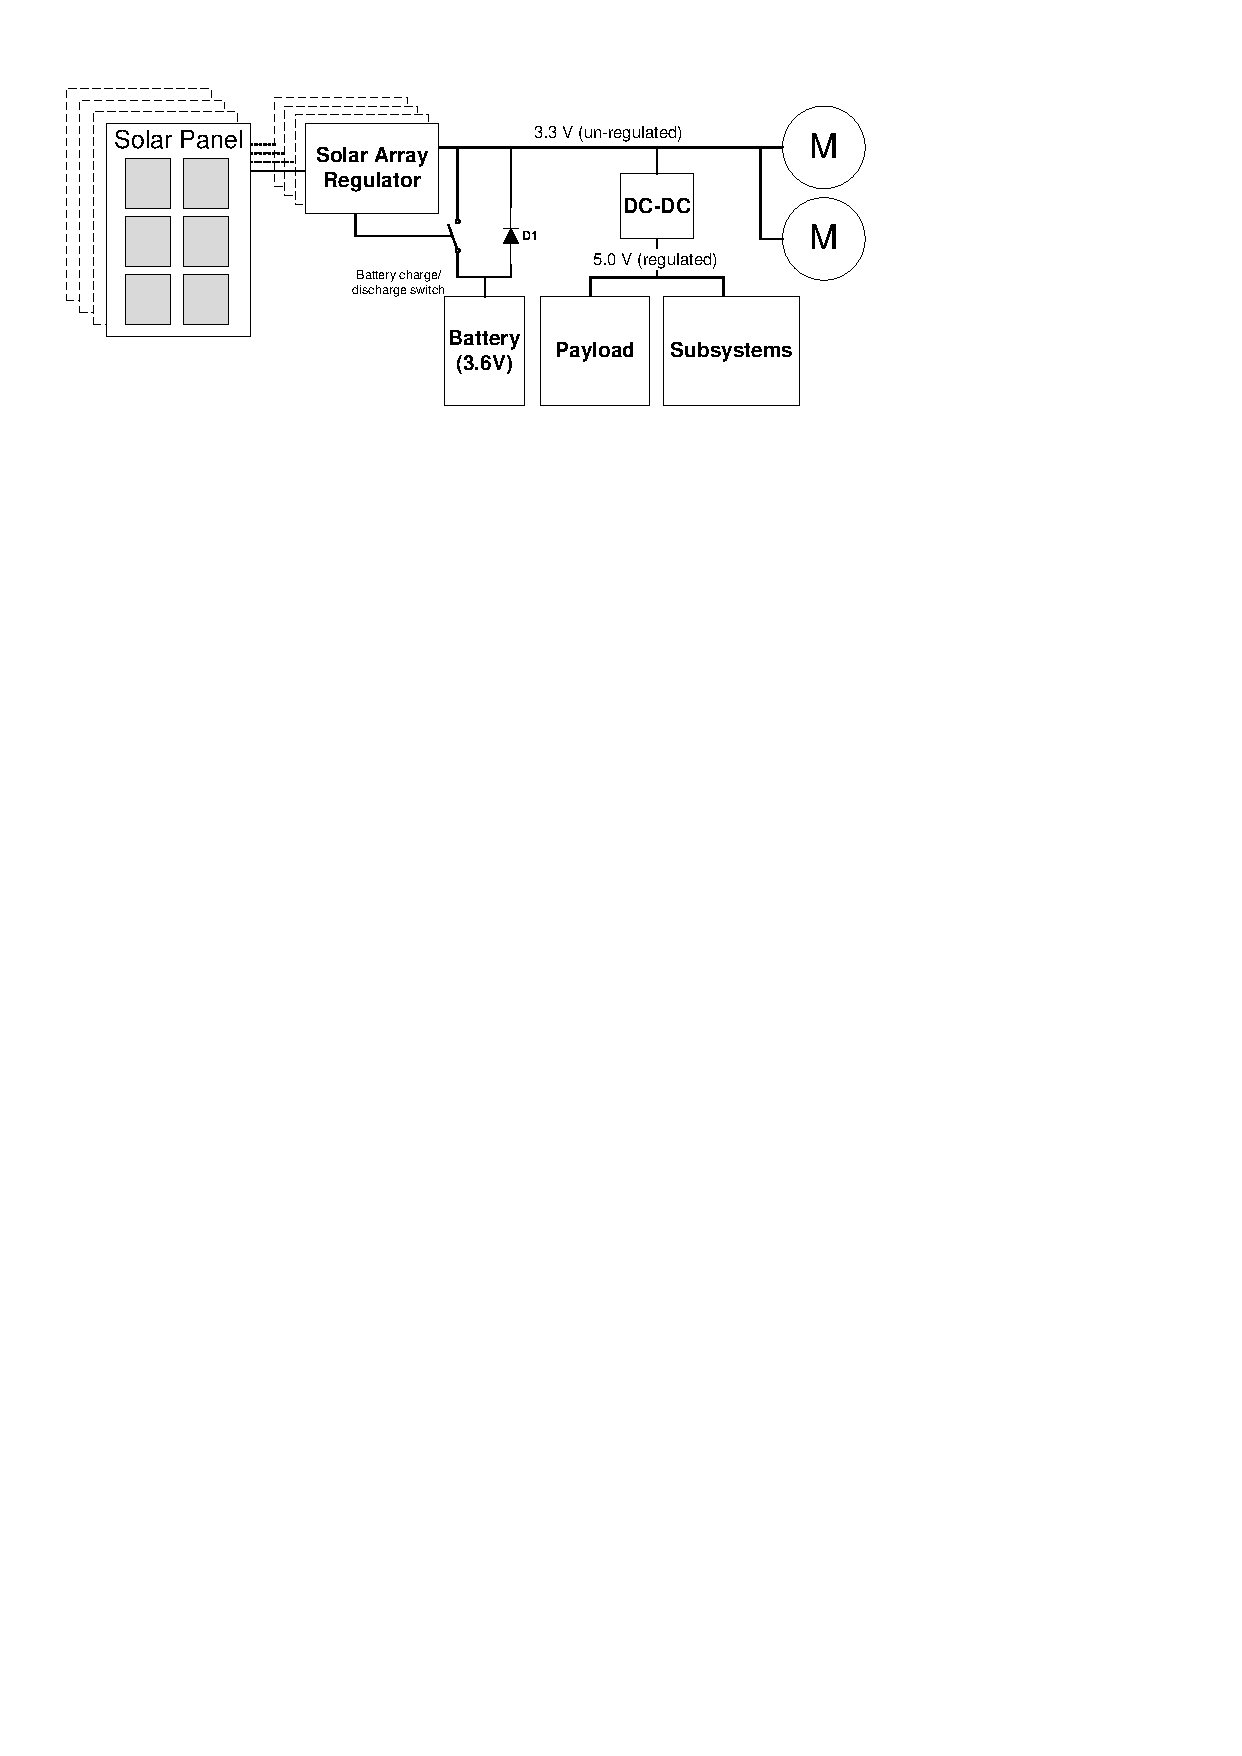
\includegraphics[scale=1]{figures/fig_PDR_EPSdiagram}
\caption{\ac{EPS} system diagram}
\label{fig:EPSdiagram}
\end{figure}
%
%
\subsection{Feasibility Study and Risk Analysis}
%How feasible is it to successfully implement the chosen concept? – Which potential issues/challenges might occur?
%
\subsubsection*{MPPT Regulator}
The \ac{MPPT} regulator is a relative large and complicated circuit requiring significant amount of man-hours to design, build and test. The responsible team has previous practical experience with both \acp{SAR} and \acp{MPPT} which is believed to drastically reduce the implementation time. With the \ac{MPPT} regulator, it is proposed first to build the DC-DC converter with output voltage control(feedback) thus resembling the shunt-regulator in functionality only with a few percent higher losses due to the DC-DC converter. This design allows one regulator to operate all four solar panels, since the \ac{MPPT} circuit is not yet included. Using this approach, it will be faster to build a first-prototype regulator, working as a backup plan, should the full \ac{MPPT} regulator prove to complicated to implement within the given project constraints. As a third backup, the extremely simple, but crude Zener-diode regulator can be implemented within very shot time, to provide a minimum amount of power.
%
\subsubsection*{Li-ion Battery}
Li-ion battery technology is widely spread used technology for modern computers and electronics. However, the technology requires more sophisticated protection circuitry against over-charge/discharge conditions, which can lead to a major system failure and potentially pose a safety risk. Extensive testing and use of application procedures should be applied.
%
\subsubsection*{Solar Arrays}
The solar arrays are the major contribution to the \ac{EPS} cost and mass budget. The proposed solar cells, \cite{MC_Solar_Cell}, list very promising specifications, however the credibility remains to be verified. If cheap and light-weight solar cells are not available, it will be a critical roadblock for realizing the project.
%
%
\subsection{Telemetry and Telecommands}
%What telemetries/telecommands are required/useful for the subsystem? – What data rates/sizes are required?
%
The required/recommended telemetry and telecommands, \ac{EPS} , are listed in table \ref{tab:Telemetry_Telecommands}.
%
\begin{table}[H]
\centering
\caption{Telemetry and telecommands}
\label{tab:Telemetry_Telecommands}
\begin{tabular}{|l|l|l|}
\hline
\textbf{Telemetry} & \textbf{Data rate/frequency} & \textbf{Data size} \\
\hline
Battery voltage & Every 30 sec & 1 byte \\
\hline
Solar array temperature & Every 30 sec & 1 byte\\
\hline
Solar array voltage & Every 1 sec(MPPT performance) & 2 bytes\\
\hline
Solar array current & Every 1 sec(MPPT performance) & 2 bytes\\
\hline%\hline
%\textbf{Telecommands} & \textbf{Parameters} & \textbf{Valid input range}\\
%set-output-voltage & $<voltage>[1 byte]$ & $0;255 (=???\,V$)\\
%\hline
\end{tabular}
\end{table}
%
\subsection{External Interfaces}
%How are the external interfaces implemented for the mechanics, power, communication etc.?
%
The interfaces of the \ac{EPS} external are listed in table \ref{tab:external_interfaces}.
%
\begin{table}[H]
\centering
\caption{External interfaces}
\label{tab:external_interfaces}
\begin{tabular}{m{0.35\textwidth}m{0.55\textwidth}}
\hline
\textbf{External interface} & \textbf{Implementation}\\
\hline
Solar array mounting to rigid ballon structure & Screws and bolts\\[2mm]
DC-DC regulators & Mounted on PCB which sits in system housing. Thermal contact points should be included, to remove internal heat dissipation.\\[2mm]
Voltage/current sensor telemetry & Analog signals to Microcontroller\\[2mm]
%Output voltage control(reference voltage setpoint) & Analog signal from Microcontroller\\[2mm]
Payload supply voltages & $3.3\,V$(unregulated) and $5.0\,V$(regulated)\\[2mm]
\hline
\end{tabular}
\end{table}